\documentclass[aspectratio=169,10pt]{beamer}

\usepackage[T1]{fontenc}
\usepackage{lmodern}
\usepackage{graphicx}
\graphicspath{{images/}}

\definecolor{Navy}{HTML}{172D45}
\definecolor{Teal}{HTML}{087F8C}
\definecolor{Muted}{HTML}{506175}
\definecolor{Amber}{HTML}{A65420}
\definecolor{Pale}{HTML}{EEF6F6}

\setbeamercolor{normal text}{fg=Navy,bg=white}
\setbeamercolor{structure}{fg=Teal}
\setbeamercolor{frametitle}{fg=Navy,bg=white}
\setbeamertemplate{navigation symbols}{}
\setbeamertemplate{frametitle}{%
  \vspace{2mm}\insertframetitle\par\vspace{1mm}%
  {\color{Teal}\rule{\textwidth}{0.65pt}}\vspace{-1mm}}
\setbeamersize{text margin left=7mm,text margin right=7mm}
\setbeamertemplate{footline}{%
  \hspace{7mm}\scriptsize Helion / Group 8\hfill
  \insertframenumber\,/\,\inserttotalframenumber\hspace{7mm}\vspace{2mm}}

\newcommand{\fault}[2]{\textbf{#1}\enspace{\color{Muted}#2}\par}
\newcommand{\source}[1]{\vfill{\fontsize{6.2}{7.5}\selectfont\color{Muted}Source: #1\par}}

\begin{document}

\begin{frame}[t]{High Bandwidth Memory}
  \begin{columns}[T,onlytextwidth]
    \begin{column}{0.38\textwidth}
      \vspace{4mm}
      {\large\bfseries HBM stacks several DRAM dies into one memory package.}\par
      \vspace{5mm}
      {\small
      \textbf{TSVs} are copper paths that pass vertically through the silicon dies.\par
      \vspace{4mm}
      \textbf{Microbumps} form the electrical contacts between adjacent dies.\par
      \vspace{4mm}
      Thousands of short parallel connections provide a wide data interface and high
      bandwidth.}
    \end{column}
    \begin{column}{0.58\textwidth}
      \centering
      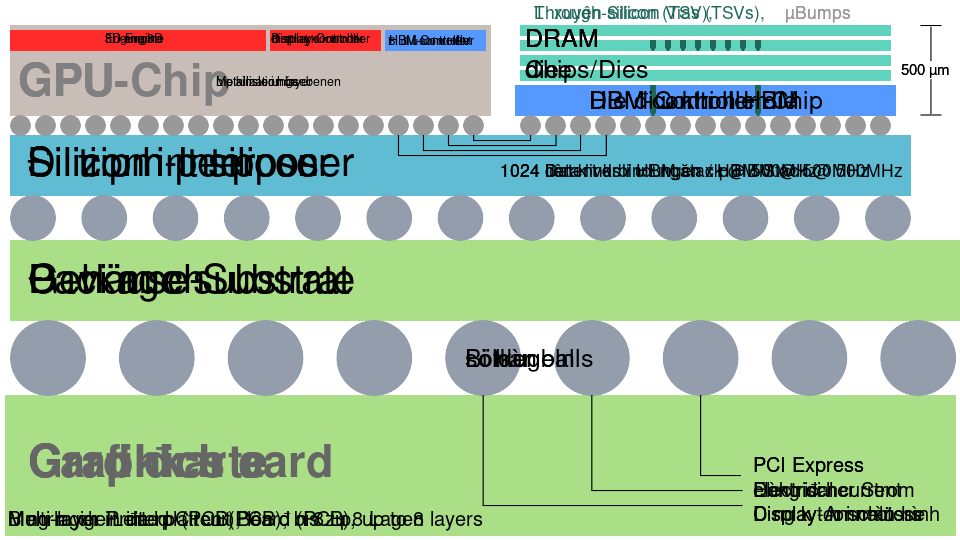
\includegraphics[width=\linewidth,trim=0 210 250 0,clip]{hbm_schematic.png}
      \vspace{2mm}
      {\small\color{Muted}Vertically stacked DRAM dies connected by TSVs and microbumps}
    \end{column}
  \end{columns}
  \source{Image: \href{https://commons.wikimedia.org/wiki/File:High_Bandwidth_Memory_schematic.svg}{ScotXW, Wikimedia Commons}, CC BY-SA 4.0. Cropped to the memory stack.}
\end{frame}

\begin{frame}[t]{Electrical and TSV-related failures}
  \begin{columns}[T,onlytextwidth]
    \begin{column}{0.39\textwidth}
      {\large\bfseries\color{Teal}Electrical}\par\smallskip
      \centering
      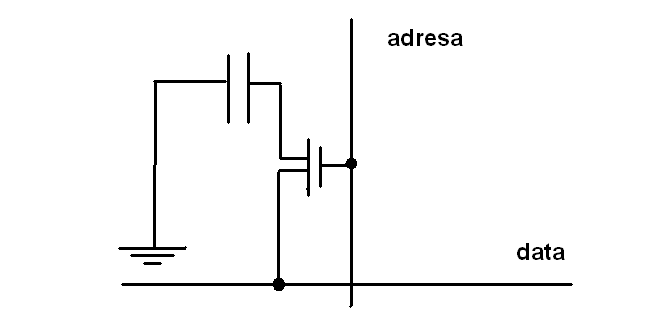
\includegraphics[width=0.92\linewidth]{dram_cell.png}
      \raggedright\vspace{2mm}
      {\small \textbf{DRAM electrical} covers internal cell and circuit faults.
      Leakage can reduce the stored charge. Circuit defects can cause abnormal current,
      timing errors or failed reads.}\par
      \vspace{2mm}
      {\scriptsize\ttfamily dram\_electrical}
    \end{column}
    \begin{column}{0.57\textwidth}
      {\large\bfseries\color{Teal}TSV-related}\par\smallskip
      \centering
      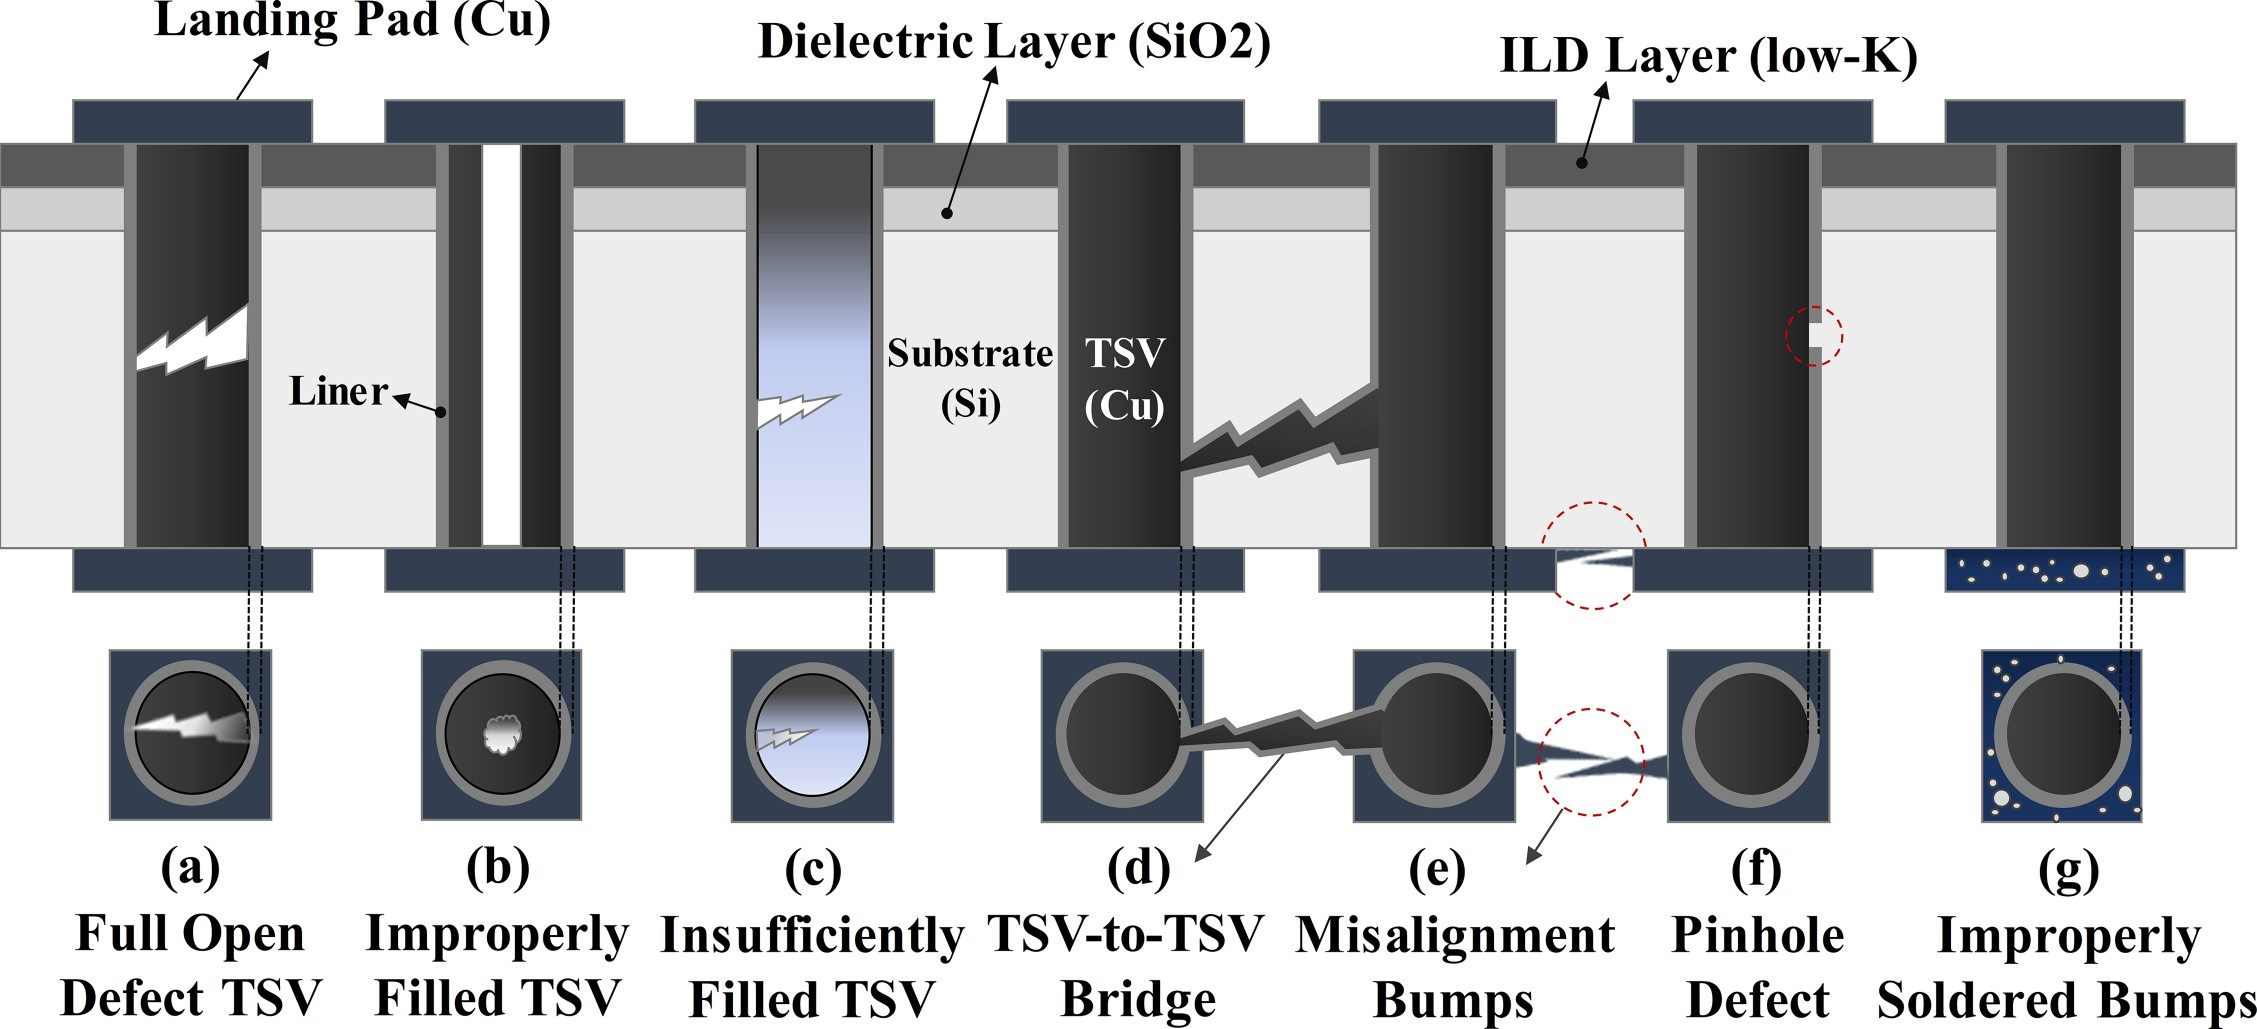
\includegraphics[width=0.98\linewidth]{tsv_page3-000.png}
      \raggedright\vspace{2mm}
      {\small A \textbf{TSV open} breaks or weakens a vertical path. A
      \textbf{TSV short} creates an unintended connection to another path or the
      surrounding material.}\par
      \vspace{2mm}
      {\scriptsize\ttfamily tsv\_open\_short}
    \end{column}
  \end{columns}
  \source{Images: \href{https://commons.wikimedia.org/wiki/File:DRAM_draft.PNG}{Cuisinier2, Wikimedia Commons}; Lee et al., \href{https://doi.org/10.1371/journal.pone.0221043}{PLOS ONE 14(8), 2019}, Fig. 1, CC BY 4.0.}
\end{frame}

\begin{frame}[t]{Microbump defects and die cracks}
  \begin{columns}[T,onlytextwidth]
    \begin{column}{0.54\textwidth}
      {\large\bfseries\color{Teal}Microbump open or bridge}\par\smallskip
      \centering
      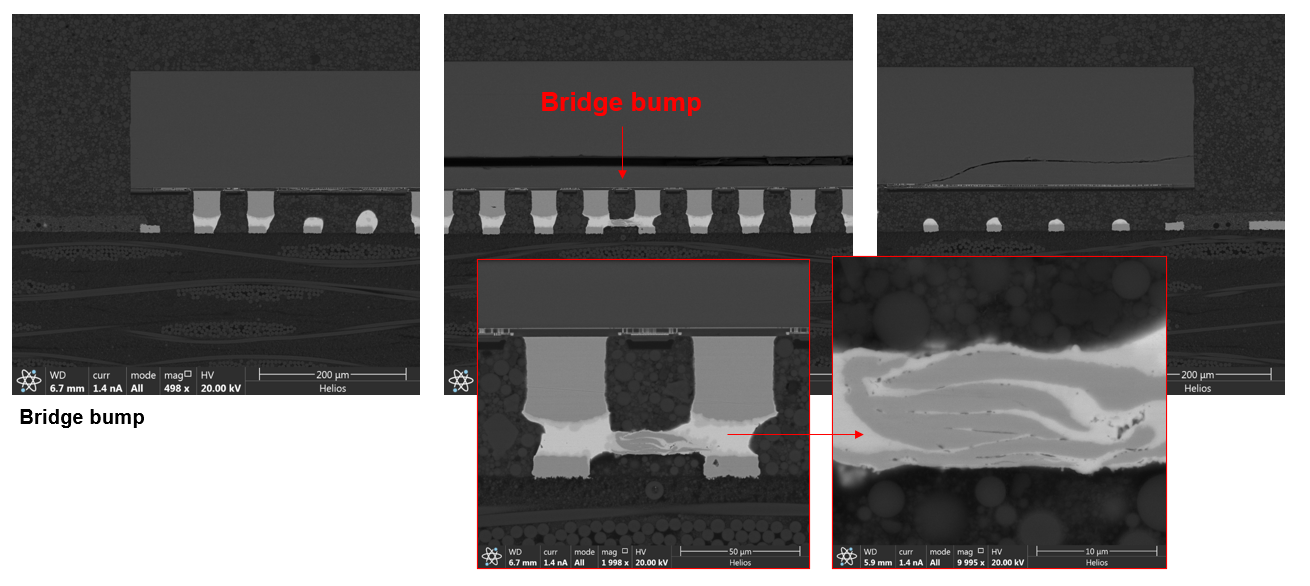
\includegraphics[width=0.98\linewidth]{microbump_bridge.png}
      \raggedright\vspace{2mm}
      {\small An \textbf{open} leaves an intended die-to-die contact disconnected.
      A \textbf{bridge} joins neighbouring contacts and creates a short.}\par
      \vspace{2mm}
      {\scriptsize\ttfamily microbump\_open\_bridge}
    \end{column}
    \begin{column}{0.42\textwidth}
      {\large\bfseries\color{Teal}Die crack}\par\smallskip
      \centering
      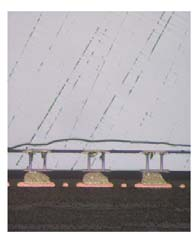
\includegraphics[height=4.18cm]{die_crack_fig-515.png}
      \raggedright\vspace{2mm}
      {\small A fracture in a silicon die can cut circuitry or grow under mechanical
      and thermal stress.}\par
      \vspace{2mm}
      {\scriptsize\ttfamily die\_crack}
    \end{column}
  \end{columns}
  \source{Images: \href{https://www.snptech.kr/archive/}{SNP Tech}, bridge-bump failure analysis; Orii et al., \href{https://imapsource.org/article/56012-scaling-challenges-of-semiconductor-packaging-in-the-era-of-big-data}{IMAPS 2013}, Fig. 3a.}
\end{frame}

\begin{frame}[t]{Warpage and interface defects}
  \begin{columns}[T,onlytextwidth]
    \begin{column}{0.46\textwidth}
      {\large\bfseries\color{Teal}Warpage}\par\smallskip
      \centering
      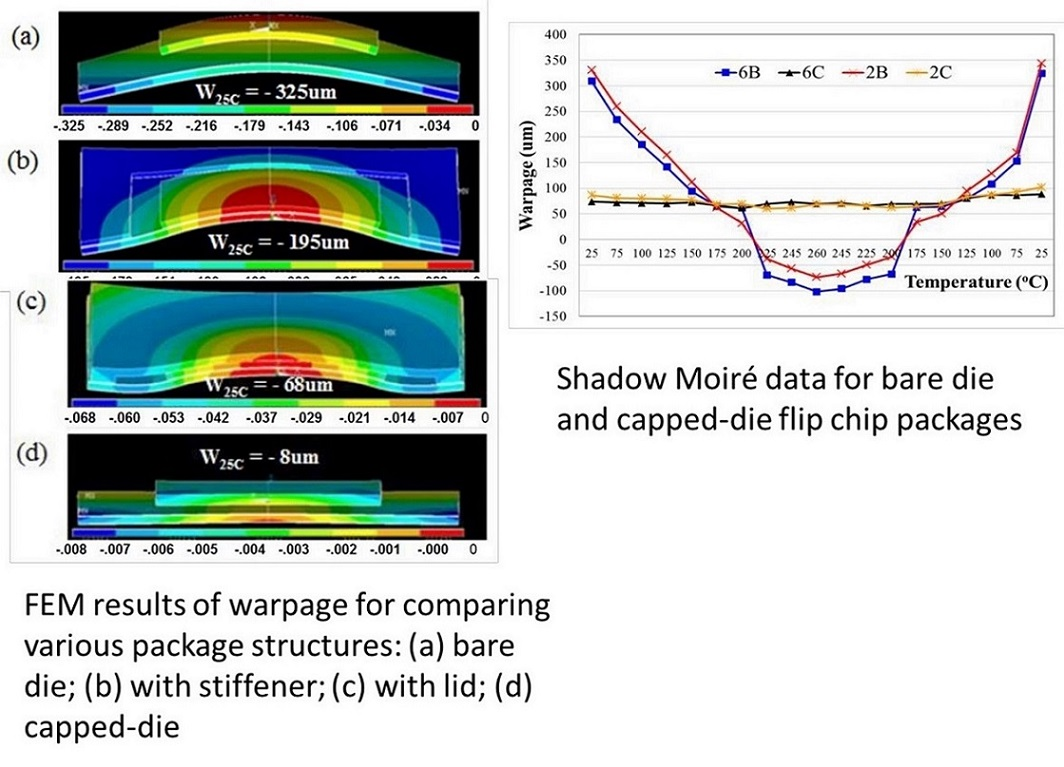
\includegraphics[height=3.7cm]{warpage.jpg}
      \raggedright\vspace{2mm}
      {\small Uneven expansion and contraction bend a die, stack or package away
      from flatness. The deformation adds stress to bonded connections.}\par
      \vspace{1mm}
      {\scriptsize\ttfamily warpage}
    \end{column}
    \begin{column}{0.50\textwidth}
      {\large\bfseries\color{Teal}Underfill void and delamination}\par\smallskip
      \centering
      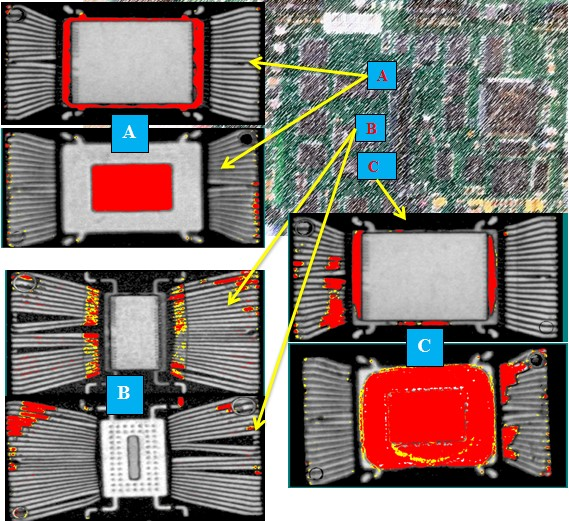
\includegraphics[height=3.7cm]{underfill_delamination.jpg}
      \raggedright\vspace{2mm}
      {\small An \textbf{underfill void} is a pocket where supporting material is
      missing. \textbf{Delamination} is separation along an interface that should
      remain bonded.}\par
      \vspace{1mm}
      {\scriptsize\ttfamily underfill\_void \qquad delamination}
    \end{column}
  \end{columns}
  \source{Images: \href{https://engineering.lamar.edu/mechanical/faculty-staff/xuejun-fan/research.html}{Lamar University, Electronic Packaging Research}; \href{https://semiengineering.com/failure-analysis-of-electronic-devices-using-scanning-acoustic-microscopy/}{Semiconductor Engineering}, scanning acoustic microscopy examples.}
\end{frame}

\end{document}
